\documentclass{article}
\usepackage[utf8]{inputenc}
\usepackage[english]{babel}
\usepackage{amsmath}
\usepackage{amssymb}
\usepackage{setspace}
\usepackage{natbib} 
\usepackage{graphicx}
\usepackage{subfig}
\usepackage{comment}
\usepackage[backgroundcolor=pink,linecolor=red]{todonotes}
\usepackage{fullpage}
\usepackage[hidelinks]{hyperref}
\usepackage{xcolor}
\usepackage{comment}

\onehalfspacing


\title{Demultiplexing Results | BIO 624}
\author{Jared Galloway}
\date{}                                           % Activate to display a given date or no date

\begin{document}
\maketitle

\newpage

\subsection*{Percentage of reads from each sample}
\begin{verbatim}
Number of hopped reads = 707740
Number of undefined reads = 30783962
Number of valid reads = 331755033

Sample Barcode	Total # Records	    Percentage of Total
GTAGCGTA	8119243	        2.447
CGATCGAT	5604966	        1.689
GATCAAGG	6587100	        1.986
AACAGCGA	8872034	        2.674
TAGCCATG	10629633	    3.204
CGGTAATC	5064906	        1.527
CTCTGGAT	34976387	    10.543
TACCGGAT	76363857	    23.018
CTAGCTCA	17332036	    5.224
CACTTCAC	4191388	        1.263
GCTACTCT	7416557	        2.236
ACGATCAG	7942853	        2.394
TATGGCAC	11184304	    3.371
TGTTCCGT	15733007	    4.742
GTCCTAAG	8830276	        2.662
TCGACAAG	3853350	        1.162
TCTTCGAC	42094112	    12.688
ATCATGCG	10087503	    3.041
ATCGTGGT	6887592	        2.076
TCGAGAGT	11741547	    3.539
TCGGATTC	4611350	        1.39
GATCTTGC	3641072	        1.098
AGAGTCCA	11316780	    3.411
AGGATAGC	8673180	        2.614
\end{verbatim}

We can see that our data contained roughly 
$331755033 / 363246735 \approx 0.91330 \approx 91.3\%$ valid reads, 
$30783962 / 363246735 \approx 0.084746 \approx 8.4\%$ undefined reads, and 
$707740 / 363246735 \approx 0.0019 \approx 0.19\%$ hopped reads. 
It appears as though the sample associated with barcode "TACCGGAT" is the most abundant at $\approx 23.018\%$ of total valid reads.

\begin{figure}[h!!]
	\center{
	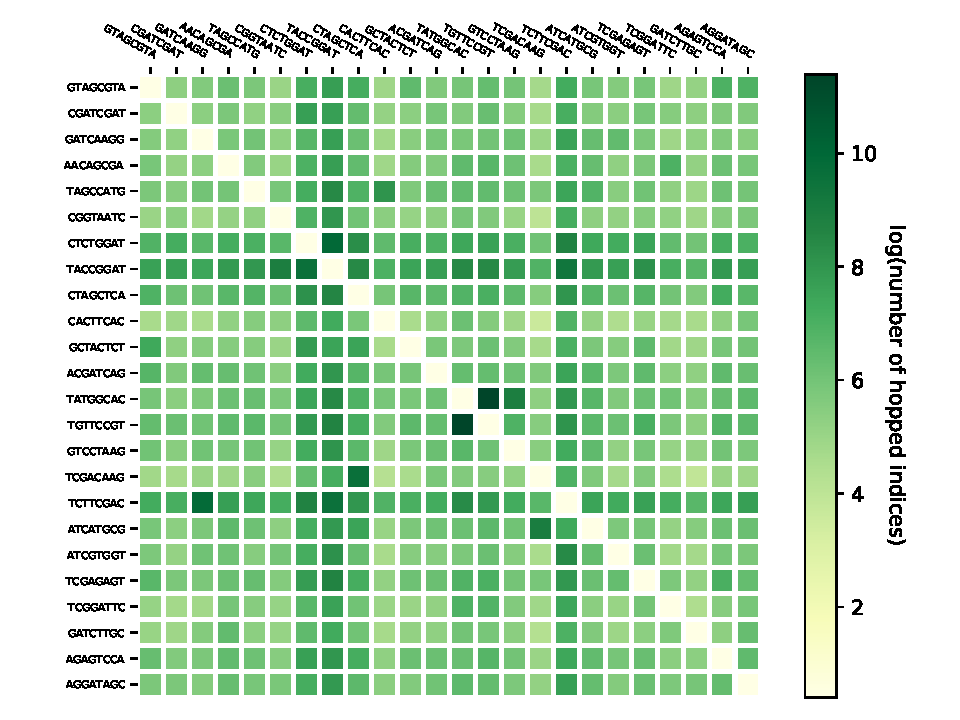
\includegraphics[width=0.8\textwidth]{../plots/heatmap.pdf}
	{}
	\caption{This figure represents the log of total number of hopped reads from one barcode, to the other in the matrix.
    For reference, $exp(log(10)) \approx 80000$}
	\label{fig:my-label} 
    }
\end{figure}

\newpage

	
\end{document}  






